\section{Data Gathering}\label{DataGathering}

For this project, we gathered data from several sources. These included several social media sites as well as the GDELT \cite{leetaru2013gdelt} events data source. In order to collect data from these sources, we initially assigned one data source to each team member to explore. Responsibility fell on each team member to collect the data and save what we considered relevant to our ElasticSearch database. This worked well for some sources that we were able to get working

\subsection{Social Media Data Gathering Strategy}

\subsubsection{Architecture}
In order to gather data from social media sources, we used several Social Media sites that provided APIs for accessing public data. These were Youtube, Mastodon, and Bluesky. We gathered data from these sources continuously using a Fission-based serverless architecture with the following components (See Figure \ref{SocialMediaGatherFig}):

\begin{enumerate}
	\item Data gathering functions: These are the actual functions in charge of gathering data from the given sources using their APIs. These functions are in charge of simply gathering the data from the source and filtering out the data that could be relevant to our use cases. These functions focus on getting real-time data from the sources as it comes in rather than batching historical data. When one of these functions gathers a record of data, it is put into a Valkey queue, which will in turn trigger the processing function via the Kubernetes Event Driven Autoscaling Fission component (Keda).
	
	\item Valkey: This is a Redis drop-in replacement we used to handle message queues used by Fission and Keda to integrate various functions in our pipeline. In this case, it serves to decouple data gathering from processing.
	
	\item Data processing function: This function is in charge of receiving data from the various social media sources, applying some transformations to the data and inserting it into our ElasticSearch indices. This function is kicked off when records are pushed to the \texttt{social-posts-index} queue on Valkey, and will process a single record in each call.
\end{enumerate}

\begin{figure}
	\begin{center}
		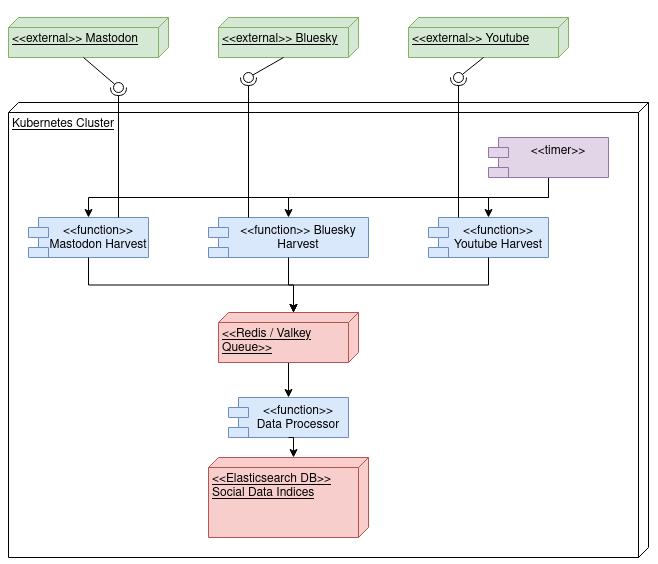
\includegraphics[width=0.65\textwidth]{./assets/SocialDataGather.png}
	\end{center}
    \caption{Architecture for Gathering Social Media Data.}
	\label{SocialMediaGatherFig}
\end{figure}

Using this message queue approach has several advantages. First, it decouples data gathering from data processing and insertion, which improves modularity and helps keep the data gathering functions lightweight and focused. Using the message queue also allows us to control the concurrency of the data processing function (which could potentially take some time) and let Valkey absorb spikes in traffic from the social media sources without throttling ingestion or overwhelming the cluster's compute capacity. If the volume of ingested data were to increase dramatically, we could scale Valkey from a single instance to a cluster and scale out the data processing function by increasing its maximum concurrency in its Fission function specification.

\subsubsection{Implementation Notes}
Within our project, we placed all our harvesting code in a single \texttt{harvesters} package both as a Python workspace and as a Fission package. This allows us to share common utilities for all functions such as credential parsing and management, and reduces the overhead of building and deploying multiple Fission packages when applying our specs. The difference between our various Social Media gathering functions is only their entrypoint and what specific submodules of our code they use.

\subsection{Social Media Providers}

\subsubsection{Mastodon}

\paragraph{Data Streaming}
One of the data sources we used was Mastodon. This is a federated network with several distinct servers, many of which have few users. In order to restrict ourselves to data specifically relevant to Australia in some way, we took the following approach:
\begin{itemize}
	\item Fetch all data from the public timeline of the Australia-focused servers \url{https://mastodon.au/} and \url{https://aus.social/}. Here we restricted ourselves to the local timeline of these services. This is to avoid data from federated servers that could come through without being relevant to Australia if we did not set this filter.
	
	\item Fetch data from the central \textit{https://mastodon.social} server and all its federated servers. In order to limit ourselves to data relevant to Australia, we fetched only data for a set of hashtags broadly related to Australia.
\end{itemize}
To harvest this data, we set up Fission functions that would run every 30 seconds for each of the three chosen Mastodon servers. The functions would use Mastodon's streaming functionality (via Server-Side Events) to stream posts as they came in for 30 seconds before shutting down for the next function call to take over.

\paragraph{Backfill}
Getting historic data from the Mastodon API was quite challenging, as it returned very few results. Because of this, we decided to use the data dump from SPARTAN used during the first assignment. This data certainly gave us a great volume of historical Mastodon posts, but unfortunately it did not overlap with the time range we were interested in, namely around the 2025 election or more recent data.

\subsubsection{Bluesky}

We designed the Bluesky ingestion component to address two complementary collection needs: \textbf{live collection}, which captures new posts continuously as they appear on the network, and \textbf{historical recovery}, which backfills posts from before the streaming deployment. This led to two modules: a \textit{streaming harvester}, built around Jetstream and WebSockets, and a \textit{historical collector}, built around authenticated HTTP search queries.
\\

\paragraph{Streaming Harvester}
For live collection, we use Bluesky Jetstream rather than polling standard REST endpoints. In the implementation, the streaming settings define a Jetstream WebSocket subscription endpoint and restrict the stream to post events in the \path{app.bsky.feed.post} collection, rather than subscribing to all repository updates. The streamer opens a WebSocket connection, continuously receives JSON messages, validates them into a \texttt{JetStreamPost} model, and retains only records whose operations are \texttt{create} or \texttt{update}. This design is consistent with the official AT Protocol / Bluesky description of Jetstream as a lightweight streaming layer built on top of the firehose, with simple JSON encoding, reduced bandwidth requirements, and filtering by collection or repository \cite{atproto2024jetstream,atproto2026streaming}.

We chose Jetstream because it is well suited to continuous real-time ingestion. However, Jetstream is primarily designed for live data rather than backfill, which is why a separate historical collection path is required \cite{atproto2024jetstream,atproto2026streaming}.

\paragraph{Streaming Filtering and Deployed Data Flow}
The streaming pipeline is not a raw mirror of all Bluesky traffic. Instead, we apply relevance filtering before forwarding data downstream. The code defines three levels of Australia-related keyword signals: \textit{strong}, \textit{medium}, and \textit{weak}. A post is accepted if it contains at least one strong keyword, at least one medium keyword, or at least two weak location-related keywords. An optional second-stage topic filter can then be applied if a keyword list is provided at runtime. This allows us to first identify broad Australian relevance and then narrow the stream to a particular policy or social topic when needed.
\\

In the deployed Fission entrypoint, \texttt{bluesky\_stream()} reads configuration from two Kubernetes secrets, namely \texttt{valkey-cfg} and \texttt{bluesky-main}. It then opens an asynchronous Valkey client and calls the \texttt{stream\_to\_vk(...)} method of \texttt{BlueskyStreamer} for a fixed runtime window. Rather than writing directly to a final analysis index, the function pushes queue messages into Valkey, where each item is formatted as \verb|{"source": "bluesky", "data": ...}|. This queue-based design decouples ingestion from downstream processing, so that indexing, schema normalization, and enrichment can be handled separately.
\\

\paragraph{Historical Collector}
Because Jetstream is fundamentally a live stream, it cannot recover older posts from before the streaming deployment started. For this reason, we implemented a dedicated historical collector. This module uses the Bluesky HTTP APIs instead of WebSockets. It authenticates with \texttt{com.atproto.server.createSession}, obtains a bearer token, and then queries \texttt{app.bsky.feed.searchPosts} over date-bounded windows \cite{bluesky2026createsession,bluesky2026searchposts}. The collector uses app-password-style credentials (\texttt{handle} and \texttt{app\_password}) rather than an interactive OAuth flow, which is appropriate for a backend harvesting process \cite{atproto2026auth,bluesky2026apihosts,bluesky2026createsession}.
\\

\paragraph{Historical Query and Windowing Strategy}
The historical collector is search-based. It starts from a default list of Australia-oriented search queries, including broad national terms such as \texttt{australia}, \texttt{australian}, and \texttt{auspol}, as well as more specific political and state-related phrases such as \texttt{federal election}, \texttt{labor party australia}, \texttt{victorian government}, \texttt{melbourne victoria}, and \texttt{queensland government}. We deliberately separate retrieval from filtering: search queries are used to maximize recall, while the strong, medium, and weak keyword lists are applied afterwards to determine whether a retrieved post is sufficiently relevant to keep. This design improves coverage without making the final retained dataset excessively noisy.
\\

A key part of the historical design is time partitioning. The collector implements a \texttt{\_three\_day\_windows(...)} helper, which splits a requested interval into sequential 3-day windows. This reduces overlap and improves coverage compared with searching across a very long period at once. The collector also exposes \texttt{page\_size}, \texttt{max\_pages}, and \texttt{sort} to control query depth within each window. In addition, it applies an explicit \texttt{cutoff\_before} timestamp so that historical ingestion only collects posts earlier than the streaming deployment boundary, reducing overlap between live and backfilled data.

\paragraph{Normalization, Deduplication, and Reliability.}
Each search result is normalized into a Bluesky-compatible structure. A deterministic document ID is then formed from \texttt{did} and \texttt{rkey}. Before sending a normalized record onward, the collector checks whether the common index (section \ref{DataProcessingCommonIndexDesign}), \texttt{social-posts-index}, already contains the corresponding \texttt{bluesky-\{did:rkey\}} document ID. If the record is new, it is pushed into the Valkey queue as a source-tagged payload. In this way, the historical collector feeds into the same downstream processing path as the live stream.
\\

To improve robustness, the historical collector supports retries for retryable HTTP status codes such as \texttt{429}, \texttt{500}, \texttt{502}, \texttt{503}, and \texttt{504}, together with exponential backoff \cite{bluesky2026ratelimits}.

\paragraph{Schema Compatibility.}
We define explicit mappings for both \path{bluesky-idx} and \path{bluesky-historical-idx}. These mappings preserve the same main Bluesky-specific structure, including \path{did}, \path{time_us}, \path{kind}, and \path{identity.handle}. They also retain a nested \path{commit} object with fields such as \path{operation}, \path{collection}, \path{rkey}, and \path{cid}, together with \path{record.text} and \path{record.createdAt}. Both mappings also include keyword arrays for matched filter terms. This schema alignment ensures that historical and live Bluesky records can be handled consistently by downstream processors and analysis workflows.

\subsubsection{Youtube}

The Youtube data is gathered using Data API v3 \cite{youtube2026dataapi} through the python library \texttt{google-api-python-client} as a scheduled Fission function, and follows the same harvester $\rightarrow$ Valkey $\rightarrow$ processor pipeline as the other providers. The API key is obtained from the Google Cloud Console (create project, enable \textit{Youtube Data API v3}, generate key under \textit{Credentials}) and stored as the secret \texttt{youtube-api-credentials}, exposed at runtime as \texttt{YOUTUBE\_API\_KEY}.

\paragraph{Queries and Customisation.}
Discovery uses \texttt{search.list} driven by a topic-to-queries dictionary defined in \texttt{youtube/defaults.py}. Pagination is limited at 30 videos per query, 50 comments per video, and 20 replies per comment.

\paragraph{Records, Validation, and Deduplication.}
The harvester collects three entities --- videos, comments, and replies --- each retaining its platform ID, parent references, text, author, like count, and publication and update timestamps; comments and replies are later enriched with a sentiment object containing label and score. 
Videos with disabled comments return HTTP 403 on \texttt{commentThreads.list}, so they are pre-filtered through a single \texttt{videos.list(part="statistics")} call that discards any with no comments, and every API call is wrapped in a try/except block so isolated failures do not abort the batch. 
Furthermore, duplicates are suppressed by using the platform ID as the ElasticSearch document ID (re-ingestion replaces the document), a per-run \texttt{seen\_ids} set, and a short-lived Valkey deduplication key. 
Because comments can be edited, the harvester preserves the last-update timestamp and overlapping windows guarantee that edits refresh the same document.

\paragraph{Indices and Valkey Pipeline.}
Data is stored in three flat indices that allow aggregations at any granularity without joins:
\begin{table}[H]
\centering
\small
\begin{tabular}{p{3.4cm}p{10cm}}
\hline
\textbf{Index} & \textbf{Fields} \\
\hline
youtube-videos-idx & video\_id, title, description, channel, channel\_id, published, topic, query \\
youtube-comments-idx & comment\_id, video\_id, video\_topic, video\_channel, video\_published, text, author, like\_count, published\_at, updated\_at, sentiment \{label, score\} \\
youtube-replies-idx & reply\_id, comment\_id, plus the same fields as comments \\
\hline
\end{tabular}
\caption{Youtube ElasticSearch indices and their fields.}
\end{table}
The harvester does not write to ElasticSearch directly; for each entity it pushes a message into the Valkey list \texttt{social-posts-index}:
\begin{verbatim}
{
    "source": "youtube",
    "data": {
        "kind": "video" | "comment" | "reply",
        "record": {...}
    }
}
\end{verbatim}
A KEDA-triggered processor consumes one message per invocation, routes it by the \texttt{kind} field, enriches text with sentiment, and writes the document, decoupling the rate-limited harvester from the heavier transformation workload.

\paragraph{Quota and Analytical Outputs.}
The API enforces 10000 units/day; \texttt{search.list} costs 100 units, the other calls cost 1 each. With the caps above and a twelve-hour trigger, usage stays within quota; if volume grew, mitigations are shrinking the query list, lowering caps, requesting a quota increase, or rotating keys. The resulting dataset supports sentiment trends per topic or channel, engagement analysis (likes, comment-to-reply ratios), ranking of channels and authors, polarity comparison between parties or leaders, keyword co-occurrence between titles and comments, and cross-platform alignment with Mastodon, Bluesky, and GDELT through shared topic and time fields.


\subsubsection{Threads}
We explored getting data from Threads required us to submit an application to Meta. Since the timeframe didn’t allow for that, we instead experimented with gathering data using web scraping. We searched for specific keywords and scrolled to the bottom of the page to load more data, repeating this process until it had loaded all the data it could find. This approach was able to gather some data, but it was not very efficient and was prone to breaking whenever Threads made changes to their frontend. For this reason, we decided to focus our efforts on the other data sources for the rest of the project. Along with the inefficiency of this approach, we also had to be careful to avoid making too many requests in a short period of time, as this could have led to our IP being blocked by Threads. We implemented some basic rate limiting in our scraping code to mitigate this risk, but it was still a concern throughout our testing. Furthermore, the addition of chromium to our package would’ve made it much heavier and more difficult to deploy, which was another reason we decided to abandon this approach.

\subsection{Additional Data Sources}

\subsubsection{GDELT}

The Global Database of Events, Language, and Tone (GDELT) monitors global news media in real-time. Our strategy for gathering this data is split into two parts: a live streaming harvester running on our serverless Fission architecture, and a separate, local script for downloading historical data.

\paragraph{Main Flow of Data.}
For live data, a Fission timer triggers the GDELT harvester every 15 minutes. It downloads the newest updates, formats them, and pushes them to our \texttt{gdelt-index} in ElasticSearch. For historical data (backfilling), we wrote a separate Python script that runs locally and uses multi-processing to download specific days in parallel. 

A simpler approach would be to use the same Fission function for both live and historical data. However, serverless functions have strict time limits and memory caps. Trying to process months of historical data on Fission would have caused timeouts and overloaded our cluster. Splitting the architecture required us to write and maintain two separate deployment strategies, which increased development time, but it ensured our live pipeline remained lightweight and fast while our local machine handled the heavy lifting of historical backfills.

\paragraph{Harvester Logic and Cross-Referencing.}
GDELT data is difficult to work with because it is split across different tables. The \textbf{Events} table contains the structural facts (who did what, and where), while the \textbf{Global Knowledge Graph (GKG)} table contains the context (emotions, tone, themes, and organizations). Our harvester downloads both tables, finds the matching records using their \texttt{CAMEOEVENTIDS} or \texttt{SOURCEURLS}, and merges them into a single JSON document. 

The easiest method would be to just upload the Events table and ignore the GKG table, or to upload them as separate documents. However, doing so would make our dashboards useless, as we needed both the geographic location (from Events) and the sentiment (from GKG) in the same query. Furthermore, instead of letting ElasticSearch generate random IDs for these documents, we engineered a deterministic ID by combining the \texttt{GlobalEventID} and the \texttt{SourceURL}. While building this matching logic was complex and required careful dictionary mapping in Python, it made our database idempotent—meaning we can accidentally run the script twice without creating duplicate records.

\paragraph{Column Selection and Data Cleaning.}
Raw GDELT files contain dozens of columns. We apply a strict \texttt{USEFUL\_COLUMNS} filter to drop most of them, keeping only core geographic data, actors, and the specific GKG sentiment and theme fields. We also run explicit data-cleaning steps, such as padding timestamps with zeros and converting missing values to \texttt{None}.

The straight forward approach is a simple ``select all'' (dumping the entire raw CSV directly into ElasticSearch). We quickly realized this would bloat our database with empty or irrelevant columns, causing unnecessary storage costs and slow queries. We also faced major bugs with data types: data libraries like Pandas try to automatically guess data types, which caused it to turn 14-digit timestamps (like \texttt{20241016000000}) into scientific floats (like \texttt{2.02E+13}), destroying our time-series data. Pandas also uses \texttt{NaN} for missing data, which causes JSON serializers to crash. Fixing this forced us to write explicit data-sanitization functions, which slowed down early development but ultimately prevented silent data corruption.

\paragraph{Fault Tolerance and Performance Optimization.}
Before uploading historical data, our script performs a final sweep to remove duplicates and saves a clean CSV backup to the local hard drive. Finally, instead of inserting records one by one, it uses ElasticSearch's \texttt{parallel\_bulk} API to upload chunks of 1500 documents at a time using multiple threads.

When dealing with massive datasets, uploading row-by-row is incredibly slow and fragile. If the internet drops after uploading 50,000 records, a simple script crashes, forcing you to start over and guess where it left off. By taking the time to implement local CSV backups, exponential retry logic, and bulk multi-threading, we made the ingestion pipeline bulletproof. This added significant complexity to our Python code, but it reduced our historical upload time from days down to hours and ensured we never lost data due to a network hiccup.

\subsubsection{Official Data}

We also incorporated sources of more official data into our study. Namely, we uploaded the 2025 election results \cite{aec_federal_election_2025} by uploading the Two-Candidate-Preferred vote counts by polling place. We hoped to use this data as a source for geographic as well as trend information, but we were unable to correlate the social media posts with geographic locations directly, since they had no geolocation data. Perhaps this could be studied across accounts in the future, by using each account's entire post history to try to determine their location and thus related them to the candidates that ran in their area.

In the end this data was still useful and insightful, as it showed the major parties and candidates we could target for further study.

\subsection{Data Collection Challenges}\label{DataGatherChallenges}

\paragraph{Data Source Access} We faced several challenges when it came to data collection from these sources. One of the first issues we encountered was access to data sources. We had initially hoped to use high-volume social media sites such as Reddit or Threads, but many platforms have tightened their API access policies, so were unable to connect to them. Instead, we were relegated to somewhat lower volume sites such as Mastodon, Bluesky, and Youtube. In the end, Bluesky proved to be our largest source of social media data by far.

\paragraph{Data Relevance} As it stands, the biggest challenge we encountered with our data sources was obtaining a large volume of \textit{relevant} data. That is, data that is relevant to Australia in some way. Once we added filtering for our specific use cases, the data volume can become quite meager. A further complication is that the data sources we had available did not have any geolocation information, such as coordinates, which meant that to determine geographic relevance we relied on keywords in the text or hashtags. This approach is overly restrictive, since posts relevant to Australia or made by people in Australia will rarely mention this fact explicitly.

Using the Mastodon streamers and the Bluesky streamer, we could get large volumes of data coming in, but most of it would not really be relevant to Australia or our use cases. In the end getting this critical mass of data while ensuring it was relevant proved to be our Achilles' heel. Perhaps our approach of filtering strictly at the source of the data was not the most effective for gathering large data volumes, as with somewhat looser filters we could still have gathered plenty of relevant historical data at the cost of some later processing and filtering.

\paragraph{Historical Data} Another great challenge was gathering \textit{historical} data from the data sources. Using the Mastodon API to obtain historical statuses was simply a non starter, as the server returned very little data from before the present even with pagination. The SPARTAN data dump gave us a great windfall in terms of volume of historical Mastodon posts, but they were unfortunately outside our desired time range. These posts were mostly from 2024 or earlier, which made them less valuable to our case study. Moreover, even some basic relevance filters like excluding posts not made from Australia-specific servers or mentioning a series of keywords discarded most of this data dump as not relevant. This left us with less than 1\% of these posts (though this was still in the hundreds of thousands). Bluesky was much more forthcoming in this regard, and we were able to get much more historical data using their API. This was still not a complete picture with all the volume we could have wanted, but it was still quite useful for our efforts.




